\section{Initial model formulation}

\subsection{General approach}

    The above findings provide sufficient information to develop a new model. In the present study, we assume EXLs induce fibre–fibre and fibre–matrix interactions that are mechanically significant. We ignore any time-dependent effects, as we have found that native and cross-linked valvular tissues exhibit minimal time-dependent effects \cite{grashow_planar_2006,grashow_biaxial_2006,stella_time_2007,eckert_biomechanical_2013}. Next, we assume that the pericardial tissues considered are only composed of collagen fibres and a matrix constituent that represents non-cross-linked and cross-linked components, and water. The contributions from elastin or other tissue components are ignored, because they have either negligible mass or stiffness. In all previous structural models of soft tissues, interactions between components (fibres, matrix) have been ignored. As we cannot assume this in the present investigation, we use the following hyperelastic general form:
        %-------------------	begin EQUATION 	-------------------%
        \begin{equation}\label{c3:eqn:41}
        \begin{aligned}
        \Psi(\mathbf{C}) = \phi_c[\Psi_c(\mathbf{C} +\Psi_\mathrm{int}(\mathbf{C}] + (1-\phi_c)\Psi_m(\mathbf{C} + p(J-1)
        \end{aligned}
        \end{equation}
        %-------------------	 end EQUATION 	-------------------%
    where $\phi_c$ is the mass fraction of the collagen fibres, $\phi_c$, $\phi_m$ and $\phi_\mathrm{int}$ are the strain energy density functions of the collagen, matrix and interaction terms, respectively, $J=\operatorname{det}(\mathbf{F})$, and $p$ is the Lagrange multiplier to enforce incompressibility. The resulting tissue-level response in terms of the second Piola-Kirchhoff stress tensor $\mathbf{S}$ is given by
        %-------------------	begin EQUATION 	-------------------%
        \begin{equation}\label{c3:eqn:42}
        \begin{aligned}
        \mathbf{S} =& 2\dpd{\psi}{\mathbf{C}} - p\mathbf{C}^{-1} \\
            =& 2\left[\phi_c\dpd{\Psi_c}{\mathbf{C}} + (1-\phi_c) \dpd{\Psi_m}{\mathbf{C}} + \phi_c \dpd{\Psi_\mathrm{int}}{\mathbf{C}}\right] - p\mathbf{C}^{-1}.
        \end{aligned}
        \end{equation}
        %-------------------	 end EQUATION 	-------------------%
        



\subsection{Accounting for changes in tissue dimensions for the collagen phase} \label{c3:sec:42}

    Results from section \ref{c3:sec:3} suggest that the native collagen fibre modulus is unaffected by cross-linking. However, the observed changes in tissue dimensions can also induce changes in tissue-level mechanical behaviour by altering the structure due to tissue shrinkage. This essentially results in a different reference configuration. There is thus a need to reformulate structural models to account for these effects directly. The formulation described in the following allows handling of changes in tissue reference state geometry. The key assumptions are:
        \begin{enumerate}
            \item Changes are due to alterations in the initial geometric configuration only, so that
            \begin{enumerate}
                \item Mass fractions of each phase remain unchanged.
                \item The internal mechanical energy remains zero. Thus, all changes in internal component configurations are not associated with any change in internal energy (which remains zero)—just initial configuration (e.g. fibre orientation, degree of undulation, thickness and length).
            \end{enumerate}
            \item Tissue dimensions and internal architecture change under the \textit{affine} kinematic assumption. Thus, the configuration of all constituent fibres in the altered reference state (after all changes in initial specimen geometry have taken place) can be predicted. Moreover, the configurational change is homogeneous, and can be thus described by a deformation gradient tensor with constant components.
            \item To be consistent with the fibre recruitment mechanisms (e.g. \cite{sacks_incorporation_2003,fata_insights_2014}), all fibres remain undulated in the new reference state.
            \item The matrix phase is unaffected by the geometric configuration changes and is referenced to $\beta_1$ (figure \ref{c3:fig:3}b) for all subsequent stress calculations.
        \end{enumerate}
        
        
    As a first step, we recast the recruitment function parameters determined in $\beta_0$ but mapped to $\beta_1$ using
        %-------------------	begin EQUATION 	-------------------%
        \begin{equation}\label{c3:eqn:43}
        \begin{aligned}
        &D_1(\mu_0, \sigma_0, \prescript{}{0}{\lambda}_{lb}, \prescript{}{0}{\lambda}_{ub}, \prescript{1}{0}{\lambda}, \prescript{}{1}{\lambda}_s) = 
            \begin{cases}
            \frac{y^{\alpha-1}(1-y)^{\beta-1}}{B(\alpha,\beta)(\prescript{}{1}{\lambda}_{ub}-\prescript{}{1}{\lambda}_{lb})} & \text{for } y \in [0,1] \\
            0 & \text{otherwise}
            \end{cases} \\
        &y=\frac{\prescript{t}{1}{\lambda}_s-\prescript{}{1}{\lambda}_{lb}}{\prescript{}{1}{\lambda}_{ub}- \prescript{}{1}{\lambda}_{lb}}, 
        \quad \prescript{}{1}{\lambda}_{ub} = \frac{\prescript{}{0}{\lambda}_{ub}}{\prescript{1}{0}{\lambda}}, 
        \quad \prescript{}{1}{\lambda}_{lb} = \frac{\prescript{}{0}{\lambda}_{lb}}{\prescript{1}{0}{\lambda}}   \\
        &\bar{\mu} =\frac{\mu - \prescript{}{0}{\lambda}_{lb}}{\prescript{}{0}{\lambda}_{ub}-\prescript{}{0}{\lambda}_{lb}},
        \quad \bar{\sigma} = \frac{\sigma}{\prescript{}{0}{\lambda}_{ub} - \prescript{}{0}{\lambda}_{lb}}, \\
        &\alpha = \frac{\bar{\mu}^2 - \bar{\mu}^3 - \bar{\sigma}^2\bar{\mu}}{\bar{\sigma}^2},  
        \quad \beta = \alpha \frac{1-\bar{\mu}}{\bar{\mu}}
        \end{aligned}
        \end{equation}
        %-------------------	 end EQUATION 	-------------------%
    where the left subscript denotes the configuration state. Note carefully that $\prescript{1}{0}{\lambda}$ will in general be a function of $\theta_1$, so that even though the collagen fibre recruitment is orientation-independent in $\beta_0$, it will have angular dependence in $\beta_1$ unless $\prescript{1}{0}{F}_{11} = \prescript{1}{0}{F}_{22}$ and $\prescript{1}{0}{F}_{12} = \prescript{1}{0}{F}_{21} = 0$. The resulting expression for the ensemble stress is
        %-------------------	begin EQUATION 	-------------------%
        \begin{equation}\label{c3:eqn:44}
        \begin{aligned}
        \prescript{t}{1}{\mathbf{S}}_c^{ens} = \phi_c\frac{\eta_c}{\prescript{t}{1}{\lambda}}
            \int_1^{\prescript{t}{1}{\lambda}} \frac{D_1(x)}{x}\left(\frac{\prescript{t}{1}{\lambda}}{x} - 1\right) \dif x
        \end{aligned}
        \end{equation}
        %-------------------	 end EQUATION 	-------------------%
    To complete the tissue-level formulation, we use the affine transformation assumption and the formulation described in \cite{fan_simulation_2014} to obtain the collagen fibre orientation distribution function $\Gamma_0$ in the native state to that in $\beta_1$ using
        %-------------------	begin EQUATION 	-------------------%
        \begin{equation}\label{c3:eqn:45}
        \begin{aligned}
        \Gamma_1[\mu_\Gamma,\sigma_\Gamma, \theta_1 = \Gamma_0[\mu_\Gamma, \sigma_\Gamma, \theta_0(\prescript{1}{0}{\mathbf{F}},\theta_1)\frac{\prescript{1}{0}{\lambda}_{\theta_0}^2}{\prescript{1}{0}{J_\mathrm{2D}}}].
        \end{aligned}
        \end{equation}
        %-------------------	 end EQUATION 	-------------------%
    Note that the angle $\theta_1$ of a fibre originally oriented at $\theta_0$ can be determined using
        %-------------------	begin EQUATION 	-------------------%
        \begin{equation}\label{c3:eqn:46}
        \begin{aligned}
        \theta_1(\prescript{1}{0}{\mathbf{F}},\theta_0) = \tan^{-1}\left(\frac{\prescript{1}{0}{F}_{21}\cos{\theta_0} + \prescript{1}{0}{F}_{22}\sin{\theta_0}}{\prescript{1}{0}{F}_{11}\cos{\theta_0} + \prescript{1}{0}{F}_{12}\sin{\theta_0}}\right)
        \end{aligned}
        \end{equation}
        %-------------------	 end EQUATION 	-------------------%
    The final form of the native collagen fibre phase expressed in the EXL state is thus
        %-------------------	begin EQUATION 	-------------------%
        \begin{equation}\label{c3:eqn:47}
        \begin{aligned}
        \prescript{t}{1}{\mathbf{S}}(\eta_c, \mu_\Gamma, \sigma_\Gamma, \mu_0, \sigma_0)& = \phi_c\frac{\eta_c}{\prescript{t}{1}{\lambda}} \int_{\theta_1} \Gamma_1(\mu_\Gamma, \sigma_\Gamma,\theta_1))
        \\
        &\left\{ \frac{D_1(\mu_0, \sigma_0, \prescript{}{0}{\lambda}_{lb}, \prescript{}{0}{\lambda}_{ub},\prescript{1}{0}{\lambda}[\theta_0(\theta_1)],x)}{x}\left(\frac{\prescript{1}{0}{\lambda}}{x} - 1\right)\dif x\right\}\mathbf{n}_1\otimes\mathbf{n}_1 \dif \theta
        \end{aligned}
        \end{equation}
        %-------------------	 end EQUATION 	-------------------%
    The above equation has a total of five fitted model parameters $\eta_c$, $\mu_\Gamma$, $\sigma_\Gamma$, $\mu_0$, and $\sigma_0$ ($\lambda_{lb}$ and $\lambda_{lb}$ are determined from the experimental data), all with a physical meaning and all referenced to $\beta_0$.

        
\subsection{The matrix phase}

    The matrix response can be estimated from the low stress region where collagen does not contribute any stress (figures \ref{c3:fig:5} and \ref{c3:fig:6}). A careful examination revealed that the toe region is a convex curve in $S-\lambda$, which is inconsistent with a neo-Hookean material model which is concave in $S-\lambda$ (figure \ref{c3:fig:6}). While we have used an exponential isotropic function for the matrix before \cite{sacks_structural_2000}, we considered the Yeoh model but found it unable to fit the data. Therefore, we developed a modified Yeoh model as
        %-------------------	begin EQUATION 	-------------------%
        \begin{equation}\label{c3:eqn:48}
        \begin{aligned}
        \Psi_m(\mathbf{C}) =& \frac{1}{2}\frac{\mu_a}{a}(I_1 - 3)^a + \frac{1}{2}\frac{\mu_b}{b}(I_1 - 3)^b  \\
        \mathbf{S}_m =& \left(\mu_a(I_1 - 3)^{a-1} + \mu_b(I_1 - 3)^{b-1}\right)(\mathbf{I} - C_{33}\mathbf{C}^{-1}), \\
        &\quad\quad \text{with } 1<a<b, \quad a\times b < 2
        \end{aligned}
        \end{equation}
        %-------------------	 end EQUATION 	-------------------%
    When applied to all pre-transition mechanical data (i.e. from all protocols and where there is no collagen fibre contribution), this form was found to fit the low-stress data quite well (figure \ref{c3:fig:6}).
    

%%%%%%%%%%%%%%%%%%%%	begin FIGURE 	%%%%%%%%%%%%%%%%%%%%
\begin{figure}
\centering
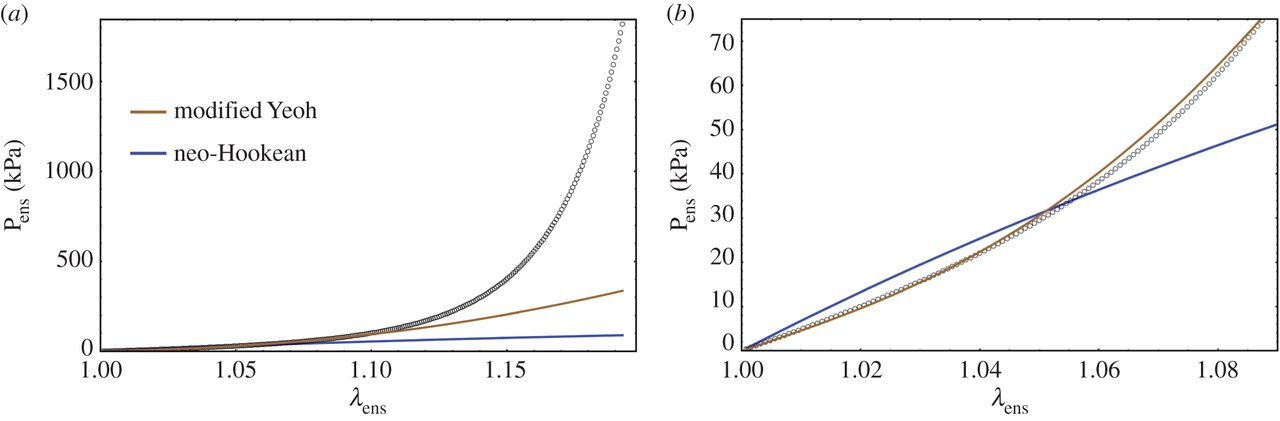
\includegraphics[width=\textwidth]{Images/chapter3/F6large.jpg}
\caption{A representative fibre-ensemble stress–strain (in $P_\mathrm{ens}-\lambda_\mathrm{ens}$)  for EXL treated bovine periardium, and (b) a close-up of the low stress region. A careful examination revealed that the toe region suggests that a modified Yeoh model was necessary to accurately capture its response (equation \ref{c3:eqn:48}) due to the convexity of the response.}
\label{c3:fig:6}
\end{figure}
%%%%%%%%%%%%%%%%%%%%	 end FIGURE 	%%%%%%%%%%%%%%%%%%%%
    
    
\subsection{Interactions}
        
    Our key working assumption is that all fibre–fibre and fibre–matrix interactions can be represented at the fibre-ensemble level. This is done to simplify the model formulation, and further since the exact micromechanical mechanisms of cross-linking have yet to be determined. Based on the form assumed in equation \ref{c3:sec:42}, we now have the ability to estimate the form and magnitude of the fibre-ensemble interactions from the fibre-ensemble data using $\mathbf{S}_\mathrm{int} \approx \mathbf{S}_\mathrm{ens} - 1/\phi_c(\phi_c \mathbf{S}_c + (1 - \phi_c)\mathbf{S}_m)$, where $\mathbf{S}_\mathrm{ens}$ is the ensemble stress (figure \ref{c3:fig:5}). Note here that the collagen stress Embedded Image and is thus the contribution of the collagen fibres expressed in the EXL configuration $\beta_1$ using equation \ref{c3:eqn:47}. This approach allowed us to exploit the matched native–EXL mechanical data by fitting the native responses then mapping them to the EXL state, so that they are a known quantity rather than one that required data fitting. Results of this analysis indicated some intriguing results. First, while the collagen phase contributed substantially to the total ensemble stress, it was only about 50\%, and the matrix only about 20\%. This revealed that the remaining approximately 30\% portion of the total ensemble stress must be a result of the interaction mechanisms.
    
    
    To model the interactions, we first consider two fibre ensembles with orientation vectors $\mathbf{n}_0(\alpha)$ and $\mathbf{m}_0(\beta)$ in the reference configuration (figure \ref{c3:fig:7}). These two ensembles can mechanically interact by elongation and relative rotation. Kinematically, these mechanisms can be captured using the pseudo-invariant $I_8$ \cite{holzapfel_nonlinear_2000,merodio_influence_2006} 
        %-------------------	begin EQUATION 	-------------------%
        \begin{equation}\label{c3:eqn:49}
        \begin{aligned}
        I_8 &= \mathbf{n}_0\cdot\mathbf{C}\mathbf{m}_0 = \cos(\theta)\lambda_\alpha\lambda_\beta \\
        \cos(\theta) &= \frac{\mathbf{n}_0\cdot\mathbf{m}_0}{\lambda_\alpha\lambda_\beta}, \quad \lambda_\alpha=\sqrt{\mathbf{n}_0\cdot\mathbf{C}\mathbf{n}_0}, \quad \lambda_\alpha=\sqrt{\mathbf{m}_0\cdot\mathbf{C}\mathbf{m}_0} 
        \end{aligned}
        \end{equation}
        %-------------------	 end EQUATION 	-------------------%
    Note that we can also use $I_8^\prime = I_8  - I_8^0$ \cite{merodio_influence_2006} to account for the relative change in fibre rotations if necessary. Thus, $i_8$ can be considered the product of an extensional term $\lambda_\alpha \lambda_\beta$ and a rotational term $\cos(\theta)$. We consider two sub-aspects of ensemble-level effects: intra- and inter-ensemble levels. The intra-ensemble incorporates all fibre–fibre interactions that occur within a single ensemble and are limited to extensional effects only. By contrast, inter-ensemble effects can include both extensional and rotational effects.
    
    
%%%%%%%%%%%%%%%%%%%%	begin FIGURE 	%%%%%%%%%%%%%%%%%%%%
\begin{figure}
\centering
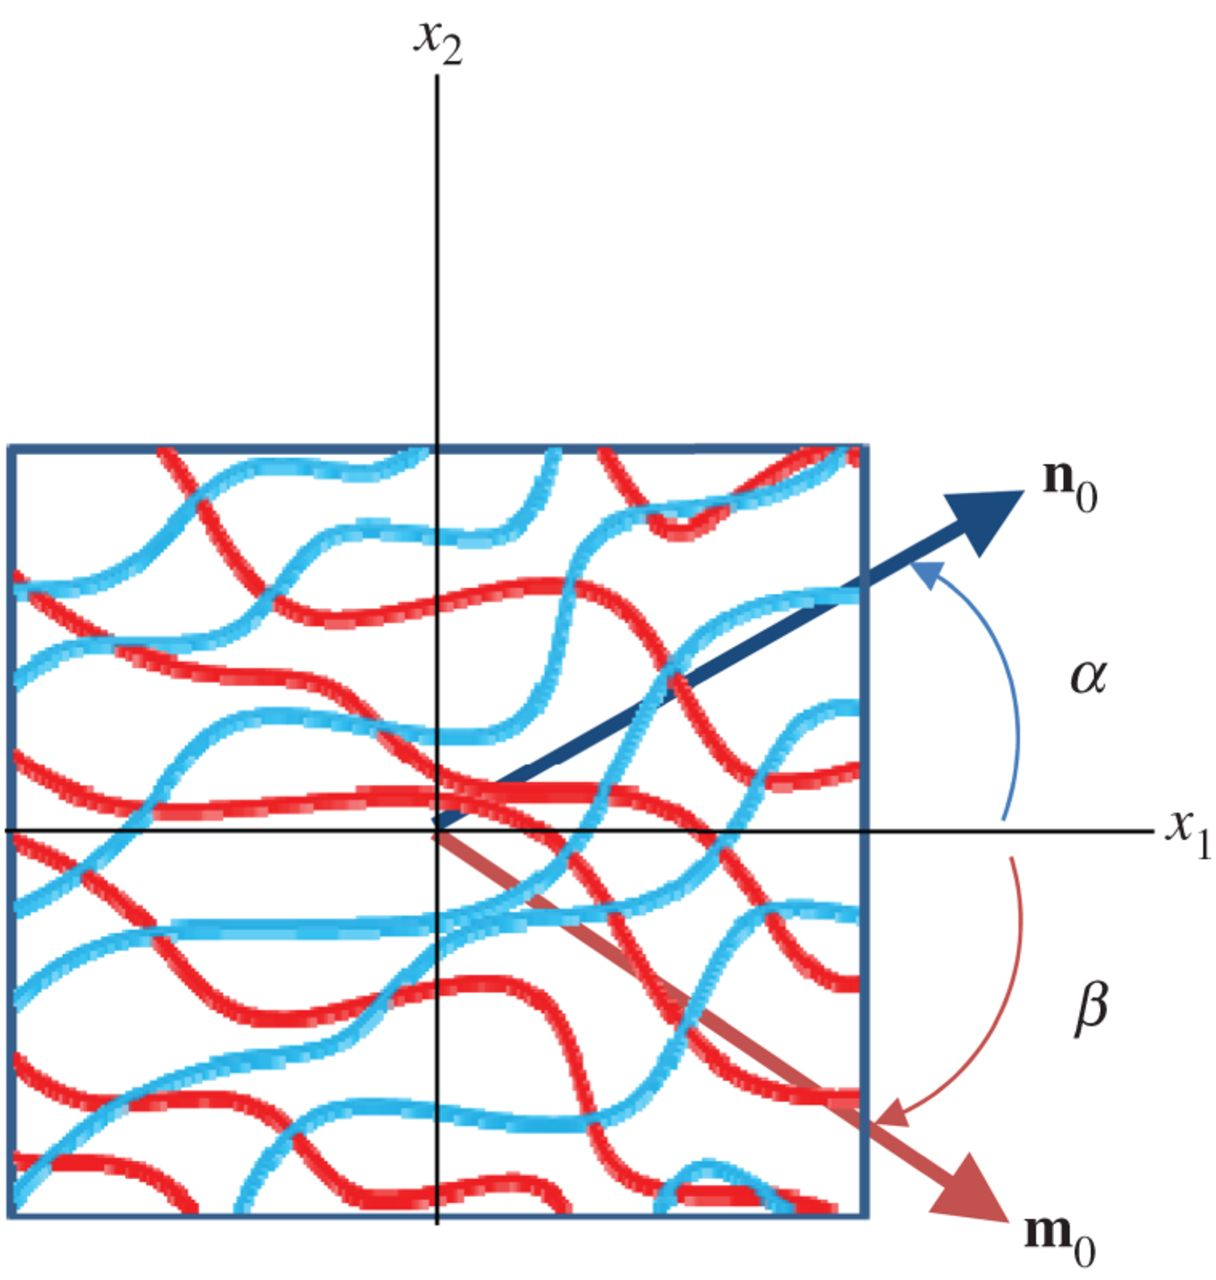
\includegraphics[width=3in]{Images/chapter3/F7large.jpg}
\caption{A schematic of two collagen fibre ensembles with respective orientations $\alpha$ and $\beta$ (not restricted to be symmetric about the $X_1$-axis) with associated orientation vector $\mathbf{n}_0$ and $\mathbf{m}_0$ in the reference configuration.}
\label{c3:fig:7}
\end{figure}
%%%%%%%%%%%%%%%%%%%%	 end FIGURE 	%%%%%%%%%%%%%%%%%%%%
    
    
    To best capture these phenomena, we do not use $I_8$ directly but rather the following forms. The results for the ensemble stress suggest that the interaction terms are exponential in character (figure \ref{c3:fig:8}). Thus, for the extensional intra-ensemble effects we use
        %-------------------	begin EQUATION 	-------------------%
        \begin{equation}\label{c3:eqn:410}
        \begin{aligned}
        \Psi_\mathrm{int}^e(\mathbf{C}) = \frac{c_0}{4}\int_\theta\Gamma(\theta)\left[e^{c_1(\lambda-1)^2} - 1\right]\dif \theta
        \end{aligned}
        \end{equation}
        %-------------------	 end EQUATION 	-------------------%
    where $\lambda = \sqrt{\mathbf{n}_0\cdot\mathbf{C}\mathbf{n}_0} = \sqrt{I_4}$ and $c_0$, $c_1$ are constants, and the associated single ensemble stress extensional interaction is
        %-------------------	begin EQUATION 	-------------------%
        \begin{equation}\label{c3:eqn:411}
        \begin{aligned}
        \mathbf{S}_\mathrm{int}^e =& 2\dpd{\Psi(\mathbf{C})}{\mathbf{C}} = 2 \dpd{\Psi(\lambda)}{\lambda}\dpd{\lambda}{\mathbf{C}}
        = \int_\theta \Gamma(\theta)\left[\frac{c_0c_1(\lambda-1)e^{c_1(\lambda-1)^2}}{\lambda}\mathbf{n}_0\otimes\mathbf{n}_0\right]\dif \theta
        \end{aligned}
        \end{equation}
        %-------------------	 end EQUATION 	-------------------%
    Next, for the extensional inter-ensemble interactions, we use a similar form
        %-------------------	begin EQUATION 	-------------------%
        \begin{equation}\label{c3:eqn:412}
        \begin{aligned}
        \Psi_\mathrm{int}^{ee}(\mathbf{C}) = \frac{d_0}{4}\int_\alpha\int_\beta\Gamma(\alpha)\Gamma(\beta)\left[e^{d_1(\lambda_\alpha\lambda_\beta-1)^2} - 1\right]\dif \alpha \dif\beta
        \end{aligned}
        \end{equation}
        %-------------------	 end EQUATION 	-------------------%
    where $d_0$ and $d_1$ are parameters, with associated stresses
        %-------------------	begin EQUATION 	-------------------%
        \begin{equation}\label{c3:eqn:413}
        \begin{aligned}
        \mathbf{S}_\mathrm{int}^e =& \int_\alpha\int_\beta \Gamma(\alpha)\Gamma(\beta) \\
        &\times\left[d_0d_1(\lambda_\alpha\lambda_\beta-1)e^{d_1(\lambda_\alpha\lambda_\beta-1)^2}\left(\frac{\lambda_\beta}{\lambda_\alpha}\mathbf{n}_0\otimes\mathbf{n}_0 + \frac{\lambda_\alpha}{\lambda_\beta}\mathbf{m}_0\otimes\mathbf{m}_0\right)\right]\dif\alpha\dif\beta
        \end{aligned}
        \end{equation}
        %-------------------	 end EQUATION 	-------------------%


%%%%%%%%%%%%%%%%%%%%	begin FIGURE 	%%%%%%%%%%%%%%%%%%%%
\begin{figure}
\centering
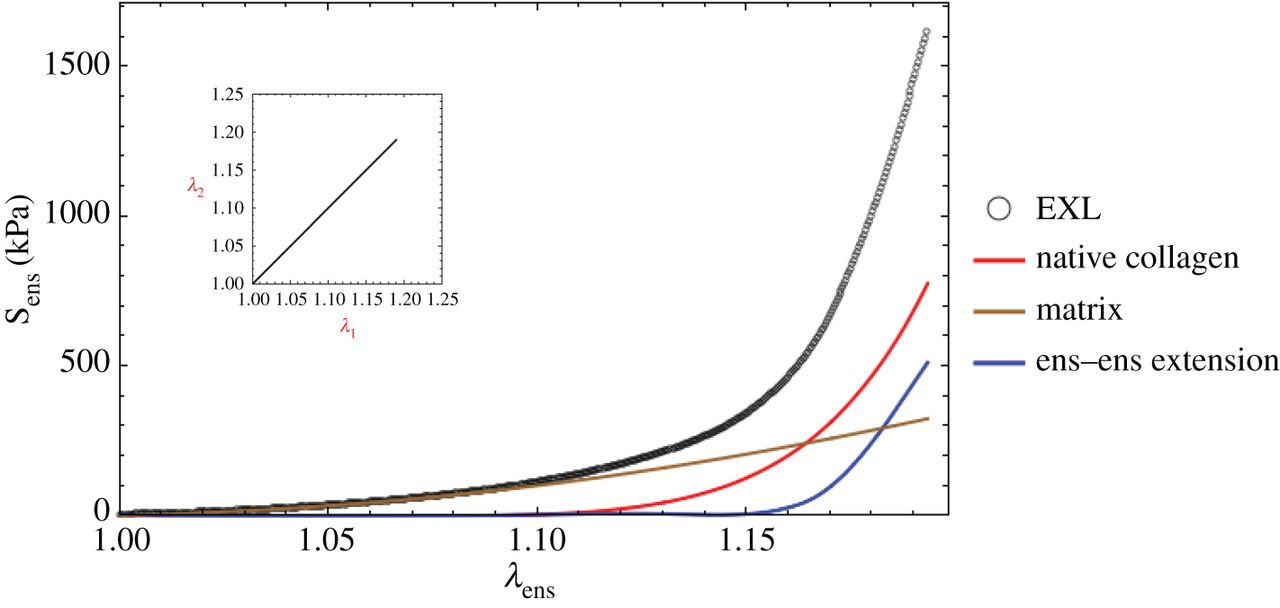
\includegraphics[width=\textwidth]{Images/chapter3/F8large.jpg}
\caption{Representative final model results (equation \ref{c3:eqn:53}) for a single fibre-ensemble stress–strain (in $S_\mathrm{ens}-\lambda_\mathrm{ens}$) response for EXL treated bovine pericardium. All model components contributed signficantly to the total stress. Surprisingly, while the collagen phase produced the greatest contribution, the interaction term was of comparable magnitude. }
\label{c3:fig:8}
\end{figure}
%%%%%%%%%%%%%%%%%%%%	 end FIGURE 	%%%%%%%%%%%%%%%%%%%%
    
    Note that the exponential term was set to zero if $\lambda_\alpha\lambda\beta<1$ In this approach, we integrate over all ensembles, weighted by their respective orientation distribution functions, to obtain the total contribution.
    
    
    Next, we developed a rotational pseudo-invariant defined as the change in the cosine between the two ensemble fibre directions, which is simply
        %-------------------	begin EQUATION 	-------------------%
        \begin{equation}\label{c3:eqn:414}
        \begin{aligned}
        I_\mathrm{int}^r(\alpha,\beta) = \frac{I_8}{\lambda_\alpha\lambda\beta} - \mathbf{n}_0\cdot\mathbf{m}_0 = \cos{\theta}-\cos{\theta_0}\approx \Delta\theta.
        \end{aligned}
        \end{equation}
        %-------------------	 end EQUATION 	-------------------%
    Using $\Psi_\mathrm{int}^r(\mathbf{C}) = \frac{\eta^r}{4}(I_\mathrm{int}^r)^2$ it can be shown that for planar distributed fibre ensembles the stress tensor is
        %-------------------	begin EQUATION 	-------------------%
        \begin{equation}\label{c3:eqn:415}
        \begin{aligned}
        \mathbf{S}_\mathrm{int}^r =& \eta^r \int_\alpha\int_\beta \Gamma(\alpha)\Gamma(\beta) \frac{I_\mathrm{int}^r(\alpha,\beta)}{\lambda_\alpha\lambda_\beta}  \\
        &\left[\left(\mathbf{m}_0\otimes\mathbf{n}_0 + \mathbf{n}_0\otimes\mathbf{m}_0\right)
        - I_8
        \left(\frac{\mathbf{n}_0\otimes\mathbf{n}_0}{\lambda_\alpha^2} + \frac{\mathbf{m}_0\otimes\mathbf{m}_0}{\lambda_\beta^2}\right)\right]\dif\alpha\dif\beta
        \end{aligned}
        \end{equation}
        %-------------------	 end EQUATION 	-------------------%
    Combining equations \ref{c3:eqn:47}\ref{c3:eqn:48}\ref{c3:eqn:411}\ref{c3:eqn:413}\ref{c3:eqn:415}, we obtain the final form of the full model stress as
        %-------------------	begin EQUATION 	-------------------%
        \begin{equation}\label{c3:eqn:416}
        \begin{aligned}
        \mathbf{S} =& \phi_c\mathbf{S}_c(\eta_c, \mu_\Gamma, \sigma_\Gamma, \mu_0, \sigma_0) + (1-\phi_c)\mathbf{S}_m(\mu_a, \mu_b, a, b) \\
        &+ \phi_c[\mathbf{S}_\mathrm{int}^e(c_0,c_1) + \mathbf{S}_\mathrm{int}^{ee}(d_0,d_1) + \mathbf{S}_\mathrm{int}^r(\eta^r)] - p\mathbf{C}^{-1}
        \end{aligned}
        \end{equation}
        %-------------------	 end EQUATION 	-------------------%
    
        
        
        